\section{Cơ sở lý thuyết}

Phần này trình bày các nền tảng toán học của tính toán tensor, bao gồm định nghĩa, các phép toán cơ bản, và các phương pháp phân rã tensor quan trọng. Các khái niệm này là cơ sở lý thuyết cho việc áp dụng tensor vào học sâu và trí tuệ nhân tạo \cite{kolda2009tensor, chrysos2025tensor}.

%%============================================================
\subsection{Tensor và cấu trúc đa chiều}
%%============================================================

\subsubsection{Tích tensor}

Trước khi định nghĩa tensor, ta cần hiểu \textit{tích tensor} (tensor product) -- phép toán đại số tuyến tính tạo ra không gian mới từ hai không gian vector.

\begin{definition}[Tích tensor của không gian vector]
Cho hai không gian vector $V$ và $W$ trên trường $\mathbb{R}$. \textit{Tích tensor} $V \otimes W$ là không gian vector được sinh bởi tập các ký hiệu hình thức $\mathbf{v} \otimes \mathbf{w}$ (với $\mathbf{v} \in V$, $\mathbf{w} \in W$), thỏa mãn các quan hệ song tuyến tính:
\begin{align}
    (\mathbf{v}_1 + \mathbf{v}_2) \otimes \mathbf{w} &= \mathbf{v}_1 \otimes \mathbf{w} + \mathbf{v}_2 \otimes \mathbf{w}, \\
    \mathbf{v} \otimes (\mathbf{w}_1 + \mathbf{w}_2) &= \mathbf{v} \otimes \mathbf{w}_1 + \mathbf{v} \otimes \mathbf{w}_2, \\
    (\lambda \mathbf{v}) \otimes \mathbf{w} &= \mathbf{v} \otimes (\lambda \mathbf{w}) = \lambda(\mathbf{v} \otimes \mathbf{w}).
\end{align}
Nếu $\{\mathbf{e}_i\}_{i=1}^m$ và $\{\mathbf{f}_j\}_{j=1}^n$ lần lượt là cơ sở của $V \cong \mathbb{R}^m$ và $W \cong \mathbb{R}^n$, thì $\{\mathbf{e}_i \otimes \mathbf{f}_j\}_{i,j}$ là cơ sở của $V \otimes W \cong \mathbb{R}^{mn}$.
\end{definition}

\begin{remark}
Tích tensor $\mathbf{v} \otimes \mathbf{w}$ của hai vector cột tương ứng với ma trận hạng 1 $\mathbf{v}\mathbf{w}^\top \in \mathbb{R}^{m \times n}$. Tổng quát hơn, tích tensor của $N$ không gian vector $\mathbb{R}^{I_1} \otimes \cdots \otimes \mathbb{R}^{I_N} \cong \mathbb{R}^{I_1 \times \cdots \times I_N}$ chính là không gian chứa các tensor bậc $N$.
\end{remark}

\subsubsection{Định nghĩa tensor}

\begin{definition}[Tensor bậc $N$]
Một \textit{tensor bậc $N$} (hay $N$-way tensor) là một mảng đa chiều, là phần tử của tích tensor $N$ không gian vector:
\begin{equation}
    \mathcal{X} \in \mathbb{R}^{I_1 \times I_2 \times \cdots \times I_N}.
\end{equation}
Mỗi chiều được gọi là một \textit{mode} (hay \textit{way}). Phần tử vô hướng tại vị trí $(i_1, i_2, \ldots, i_N)$ được ký hiệu $\mathcal{X}_{i_1, i_2, \ldots, i_N} \in \mathbb{R}$.
\end{definition}

Tensor tổng quát hóa các đối tượng quen thuộc: vector ($N=1$), ma trận ($N=2$), và tensor bậc cao ($N \geq 3$). Hình~\ref{fig:tensor-orders} minh họa trực quan các bậc tensor.

% --- TikZ helpers ---
\newcommand{\tfgCellW}{0.50}
\newcommand{\tfgCellH}{0.50}
\newcommand{\drawtfgface}[7]{% rows, cols, x, y, fill, draw, dashed(0/1)
  \pgfmathsetmacro{\tfgW}{#2*\tfgCellW}%
  \pgfmathsetmacro{\tfgH}{#1*\tfgCellH}%
  \draw[line width=0.55pt, fill=#5, draw=#6, rounded corners=2.5pt]
    (#3,#4) rectangle (#3+\tfgW,#4-\tfgH);
  \pgfmathtruncatemacro{\tfgRows}{#1}%
  \ifnum\tfgRows>1
    \foreach \i in {1,...,\numexpr\tfgRows-1\relax} {%
      \ifnum#7=1
        \draw[line width=0.4pt, dashed, #6!55] (#3,#4-\i*\tfgCellH) -- (#3+\tfgW,#4-\i*\tfgCellH);
      \else
        \draw[line width=0.4pt, #6!55] (#3,#4-\i*\tfgCellH) -- (#3+\tfgW,#4-\i*\tfgCellH);
      \fi
    }%
  \fi
  \pgfmathtruncatemacro{\tfgCols}{#2}%
  \ifnum\tfgCols>1
    \foreach \j in {1,...,\numexpr\tfgCols-1\relax} {%
      \ifnum#7=1
        \draw[line width=0.4pt, dashed, #6!55] (#3+\j*\tfgCellW,#4) -- (#3+\j*\tfgCellW,#4-\tfgH);
      \else
        \draw[line width=0.4pt, #6!55] (#3+\j*\tfgCellW,#4) -- (#3+\j*\tfgCellW,#4-\tfgH);
      \fi
    }%
  \fi
}
\newcommand{\drawtfgvec}[5]{% len, x, ytop, fill, draw
  \drawtfgface{#1}{1}{#2}{#3}{#4}{#5}{0}%
}
\newcommand{\drawtfgveccy}[5]{% len, x, ycenter, fill, draw
  \pgfmathsetmacro{\tfgTop}{#3+0.5*#1*\tfgCellH}%
  \drawtfgface{#1}{1}{#2}{\tfgTop}{#4}{#5}{0}%
}
\newcommand{\drawtfgtensor}[7]{% I, J, K, x, y, fill, draw
  \def\tfgOx{-0.22}\def\tfgOy{0.20}%
  \pgfmathsetmacro{\tfgW}{#2*\tfgCellW}%
  \pgfmathsetmacro{\tfgH}{#1*\tfgCellH}%
  \pgfmathtruncatemacro{\tfgDepth}{#3}%
  \pgfmathtruncatemacro{\tfgLast}{\numexpr\tfgDepth-1\relax}%
  \foreach \s in {\tfgLast,...,0} {%
    \pgfmathsetmacro{\tfgSx}{#4+(\s)*\tfgOx}%
    \pgfmathsetmacro{\tfgSy}{#5+(\s)*\tfgOy}%
    \ifnum\s=0
      \drawtfgface{#1}{#2}{\tfgSx}{\tfgSy}{#6}{#7}{1}%
    \else
      \drawtfgface{#1}{#2}{\tfgSx}{\tfgSy}{#6}{#7}{0}%
    \fi
  }%
  \pgfmathsetmacro{\tfgBx}{#4+\tfgLast*\tfgOx}%
  \pgfmathsetmacro{\tfgBy}{#5+\tfgLast*\tfgOy}%
  \draw[line width=0.45pt, dashed, #7!35]
    (#4,#5) -- (\tfgBx,\tfgBy)
    (#4+\tfgW,#5) -- (\tfgBx+\tfgW,\tfgBy)
    (#4,#5-\tfgH) -- (\tfgBx,\tfgBy-\tfgH)
    (#4+\tfgW,#5-\tfgH) -- (\tfgBx+\tfgW,\tfgBy-\tfgH);
}

\begin{figure}[h]
\centering
\begin{tikzpicture}[scale=0.88, every node/.style={font=\small}]
  % ---- Scalar (bậc 0) ----
  \drawtfgface{1}{1}{0}{0}{violet!18}{black!55}{0}
  \node[below=6pt] at (0.25,-0.75) {Scalar $\mathbb{R}$};
  \node[above=3pt, font=\tiny\color{gray}] at (0.25,0.05) {bậc 0};

  % ---- Vector (bậc 1) ----
  \begin{scope}[xshift=2.4cm]
    \drawtfgvec{4}{0}{0}{teal!22}{teal!55!black}
    \node[below=4pt] at (0.25,-2.25) {Vector $\mathbb{R}^{I}$};
    \node[above=3pt, font=\tiny\color{gray}] at (0.25,0.05) {bậc 1};
  \end{scope}

  % ---- Matrix (bậc 2) ----
  \begin{scope}[xshift=4.8cm]
    \drawtfgface{4}{3}{0}{0}{orange!22}{orange!65!black}{0}
    \node[below=4pt] at (0.75,-2.25) {Ma trận $\mathbb{R}^{I\times J}$};
    \node[above=3pt, font=\tiny\color{gray}] at (0.75,0.05) {bậc 2};
  \end{scope}

  % ---- Tensor bậc 3 ----
  \begin{scope}[xshift=8.2cm, yshift=-0.05cm]
    \drawtfgtensor{4}{3}{3}{0}{0}{pink!22}{magenta!55!black}
    \node[below=4pt] at (0.95,-2.35) {Tensor $\mathbb{R}^{I\times J\times K}$};
    \node[above=3pt, font=\tiny\color{gray}] at (0.95,0.45) {bậc 3};
  \end{scope}
\end{tikzpicture}
\caption{Minh họa các bậc tensor: scalar (bậc 0), vector (bậc 1), ma trận (bậc 2), và tensor bậc 3.}
\label{fig:tensor-orders}
\end{figure}

\subsubsection{Cấu trúc con: Fiber và Slice}

\begin{definition}[Fiber và Slice]
Cho $\mathcal{X} \in \mathbb{R}^{I_1 \times \cdots \times I_N}$.
\begin{itemize}
    \item \textit{Mode-$n$ fiber}: vector thu được bằng cách cố định tất cả các chỉ số ngoại trừ chỉ số thứ $n$. Ký hiệu $\mathcal{X}_{i_1,\ldots,i_{n-1},:,i_{n+1},\ldots,i_N} \in \mathbb{R}^{I_n}$.
    \item \textit{Slice}: ma trận thu được bằng cách cố định tất cả chỉ số ngoại trừ hai. Với $\mathcal{X} \in \mathbb{R}^{I_1 \times I_2 \times I_3}$: frontal slice $\mathcal{X}_{:,:,k} \in \mathbb{R}^{I_1 \times I_2}$, lateral slice $\mathcal{X}_{:,j,:} \in \mathbb{R}^{I_1 \times I_3}$, horizontal slice $\mathcal{X}_{i,:,:} \in \mathbb{R}^{I_2 \times I_3}$.
\end{itemize}
\end{definition}

%%============================================================
\subsection{Các phép toán cơ bản trên tensor}
%%============================================================

\subsubsection{Matricization (Unfolding)}

Matricization là phép tái định hình tensor thành ma trận bằng cách trải phẳng theo một mode, là công cụ kết nối đại số tensor với đại số tuyến tính cổ điển.

\begin{definition}[Mode-$n$ Matricization]
\textit{Mode-$n$ matricization} (hay unfolding) của $\mathcal{X} \in \mathbb{R}^{I_1 \times \cdots \times I_N}$ là ma trận $\mathbf{X}_{(n)} \in \mathbb{R}^{I_n \times I_{-n}}$, trong đó:
\begin{equation}
    I_{-n} = \prod_{k \neq n} I_k,
\end{equation}
và phần tử $\mathcal{X}_{i_1,\ldots,i_N}$ được ánh xạ tới phần tử $(i_n,\, j)$ của $\mathbf{X}_{(n)}$ với:
\begin{equation}
    j = 1 + \sum_{\substack{k=1\\k\neq n}}^{N} (i_k - 1) \prod_{\substack{m=1\\m\neq n}}^{k-1} I_m.
\end{equation}
Các mode-$n$ fiber trở thành các cột của $\mathbf{X}_{(n)}$.
\end{definition}

\begin{figure}[h]
\centering
\begin{tikzpicture}[scale=0.82, every node/.style={font=\small}]
  \pgfmathsetmacro{\tfgCy}{-0.75}

  % --- Tensor 3 x 4 x 2 ---
  \pgfmathsetmacro{\tXTop}{\tfgCy+1.5*\tfgCellH}
  \begin{scope}
    \drawtfgtensor{3}{4}{2}{0}{\tXTop}{pink!22}{magenta!70!black}
    \node[above=4pt, font=\footnotesize\bfseries] at (1.0, \tXTop+0.05)
      {$\mathcal{X}\in\mathbb{R}^{3\times 4\times 2}$};
    % mode 1
    \draw[teal, line width=0.85pt, <->, >=stealth]
      (-0.42, \tXTop+0.04) -- (-0.42, \tXTop-3*\tfgCellH-0.04)
      node[midway, left, align=right, text=teal, font=\footnotesize]
        {mode 1\\($I_1{=}3$)};
    % mode 2
    \draw[orange!85!black, line width=0.85pt, <->, >=stealth]
      (0.04, \tXTop-3*\tfgCellH-0.28) -- (4*\tfgCellW-0.04, \tXTop-3*\tfgCellH-0.28)
      node[midway, below, text=orange!85!black, font=\footnotesize]
        {mode 2 ($I_2{=}4$)};
    % mode 3
    \draw[purple!75!black, line width=0.85pt, ->, >=stealth]
      (4*\tfgCellW+0.02, \tXTop-0.02) -- (4*\tfgCellW-0.20, \tXTop+0.18)
      node[midway, right, xshift=2pt, text=purple!75!black, font=\footnotesize]
        {mode 3 ($I_3{=}2$)};
  \end{scope}

  % --- unfold ---
  \draw[->, line width=1.1pt, gray!60, >=stealth] (2.55, \tfgCy) -- (3.55, \tfgCy)
    node[midway, above=2pt, font=\footnotesize, text=gray!65] {unfold};

  % --- Ma trận 3 x 8 ---
  \begin{scope}[xshift=3.75cm]
    \pgfmathsetmacro{\mXTop}{\tfgCy+1.5*\tfgCellH}
    \drawtfgface{3}{8}{0}{\mXTop}{teal!18}{teal!65!black}{0}
    \node[above=4pt, font=\footnotesize\bfseries, text=teal] at (2.0, \mXTop+0.05)
      {$\mathbf{X}_{(1)}\in\mathbb{R}^{3\times 8}$};
    \draw[teal, line width=0.85pt, <->, >=stealth]
      (-0.42, \mXTop+0.04) -- (-0.42, \mXTop-3*\tfgCellH-0.04)
      node[midway, left, text=teal, font=\footnotesize] {$I_1{=}3$};
    \draw[teal, line width=0.85pt, <->, >=stealth]
      (0.04, \mXTop-3*\tfgCellH-0.28) -- (8*\tfgCellW-0.04, \mXTop-3*\tfgCellH-0.28)
      node[midway, below, text=teal, font=\footnotesize] {$I_2 I_3 {=} 8$};
  \end{scope}
\end{tikzpicture}
\caption{Mode-1 matricization của $\mathcal{X}\in\mathbb{R}^{3\times 4\times 2}$ thành $\mathbf{X}_{(1)}\in\mathbb{R}^{3\times 8}$: các mode-1 fiber trở thành cột của ma trận kết quả.}
\label{fig:matricization}
\end{figure}

\subsubsection{Tích ngoài (Outer Product)}

\begin{definition}[Tích ngoài tensor]
Cho các vector $\mathbf{a}^{(1)} \in \mathbb{R}^{I_1}, \ldots, \mathbf{a}^{(N)} \in \mathbb{R}^{I_N}$. \textit{Tích ngoài} của chúng là:
\begin{equation}
    \mathcal{X} = \mathbf{a}^{(1)} \circ \mathbf{a}^{(2)} \circ \cdots \circ \mathbf{a}^{(N)} \in \mathbb{R}^{I_1 \times \cdots \times I_N},
\end{equation}
với phần tử:
\begin{equation}
    \mathcal{X}_{i_1, \ldots, i_N} = a^{(1)}_{i_1} \cdot a^{(2)}_{i_2} \cdots a^{(N)}_{i_N}.
\end{equation}
Tensor thu được từ tích ngoài của $N$ vector được gọi là \textit{tensor hạng 1}.
\end{definition}

\begin{figure}[h]
\centering
\begin{tikzpicture}[scale=0.82, every node/.style={font=\small}]
  \pgfmathsetmacro{\opCy}{-1.05}
  \pgfmathsetmacro{\labelY}{0.55}

  % ===== Hàng nhãn (căn theo tâm đồ họa bên dưới) =====
  \node[text=teal, font=\footnotesize\bfseries] at (0.25, \labelY)
    {$\mathbf{a}\in\mathbb{R}^I$};
  \node[text=orange!85!black, font=\footnotesize\bfseries] at (1.30, \labelY)
    {$\mathbf{b}\in\mathbb{R}^J$};
  \node[text=magenta!70!black, font=\footnotesize\bfseries] at (2.30, \labelY)
    {$\mathbf{c}\in\mathbb{R}^K$};
  \node[text=violet!80!black, font=\footnotesize\bfseries, align=center] at (3.90, \labelY)
    {$\mathcal{X}=\mathbf{a}\circ\mathbf{b}\circ\mathbf{c}$\\[1pt]
     $\in\mathbb{R}^{I\times J\times K}$};

  % ===== Hàng đồ họa =====
  \drawtfgveccy{4}{0.00}{\opCy}{teal!28}{teal!55!black}
  \node[font=\Large] at (0.72, \opCy) {$\circ$};

  \drawtfgveccy{3}{1.05}{\opCy}{orange!28}{orange!70!black}
  \node[font=\Large] at (1.72, \opCy) {$\circ$};

  \drawtfgveccy{2}{2.05}{\opCy}{pink!30}{magenta!55!black}
  \node[font=\Large] at (2.72, \opCy) {$=$};

  % Tensor 4 x 3 x 2
  \begin{scope}[xshift=3.15cm]
    \pgfmathsetmacro{\tTop}{\opCy+2*\tfgCellH}
    \drawtfgtensor{4}{3}{2}{0}{\tTop}{violet!18}{violet!65!black}
    \node[font=\scriptsize, text=violet!75!black, align=center] at (0.75, \opCy)
      {$\mathcal{X}_{i,j,k}$\\[0pt]$= a_i b_j c_k$};
  \end{scope}
\end{tikzpicture}
\caption{Tích ngoài $\mathbf{a} \circ \mathbf{b} \circ \mathbf{c}$ tạo ra tensor hạng 1 bậc 3. Mỗi phần tử $\mathcal{X}_{i,j,k} = a_i b_j c_k$.}
\label{fig:outer-product}
\end{figure}

\subsubsection{Tích mode-$n$}

\begin{definition}[Mode-$n$ Product]
\textit{Tích mode-$n$} của $\mathcal{X} \in \mathbb{R}^{I_1 \times \cdots \times I_N}$ với ma trận $\mathbf{U} \in \mathbb{R}^{J \times I_n}$ là tensor:
\begin{equation}
    \mathcal{Y} = \mathcal{X} \times_n \mathbf{U} \in \mathbb{R}^{I_1 \times \cdots \times I_{n-1} \times J \times I_{n+1} \times \cdots \times I_N},
\end{equation}
với phần tử:
\begin{equation}
    \mathcal{Y}_{i_1,\ldots,i_{n-1},j,i_{n+1},\ldots,i_N} = \sum_{i_n=1}^{I_n} \mathcal{X}_{i_1,\ldots,i_N} \cdot U_{j,i_n}.
\end{equation}
\end{definition}

Tích mode-$n$ có biểu diễn tương đương qua matricization, là tính chất cơ bản kết nối phép toán tensor với đại số ma trận:
\begin{equation}
    \mathbf{Y}_{(n)} = \mathbf{U}\, \mathbf{X}_{(n)}.
\end{equation}

\begin{proposition}[Tính chất của tích mode-$n$]
\label{prop:mode-n}
Cho $\mathcal{X} \in \mathbb{R}^{I_1 \times \cdots \times I_N}$, $\mathbf{U} \in \mathbb{R}^{J \times I_n}$, $\mathbf{V} \in \mathbb{R}^{K \times J}$. Khi đó:
\begin{enumerate}[label=(\roman*)]
    \item \textit{(Kết hợp cùng mode)} $(\mathcal{X} \times_n \mathbf{U}) \times_n \mathbf{V} = \mathcal{X} \times_n (\mathbf{V}\mathbf{U})$.
    \item \textit{(Hoán vị khác mode)} Với $m \neq n$: $(\mathcal{X} \times_m \mathbf{A}) \times_n \mathbf{B} = (\mathcal{X} \times_n \mathbf{B}) \times_m \mathbf{A}$.
\end{enumerate}
\end{proposition}

\begin{proof}
\textit{(i)} Theo định nghĩa và biểu diễn matricization:
\begin{equation}
    ((\mathcal{X} \times_n \mathbf{U}) \times_n \mathbf{V})_{(n)}
    = \mathbf{V}\,(\mathcal{X} \times_n \mathbf{U})_{(n)}
    = \mathbf{V}\,\mathbf{U}\,\mathbf{X}_{(n)}
    = (\mathcal{X} \times_n \mathbf{V}\mathbf{U})_{(n)}.
\end{equation}

\textit{(ii)} Với $m \neq n$, tích mode-$m$ và mode-$n$ tác động lên các chiều độc lập nhau, do đó thứ tự thực hiện không ảnh hưởng tới kết quả. Cụ thể, phần tử tổng quát của cả hai vế đều bằng:
\begin{equation}
    \sum_{i_m} \sum_{i_n} \mathcal{X}_{\ldots,i_m,\ldots,i_n,\ldots} \cdot A_{j_m, i_m} \cdot B_{j_n, i_n}. \qedhere
\end{equation}
\end{proof}

%%============================================================
\subsection{Phân rã tensor}
%%============================================================

Phân rã tensor là quá trình biểu diễn một tensor bậc cao dưới dạng tổ hợp của các thành phần đơn giản hơn, cho phép nén dữ liệu và trích xuất cấu trúc tiềm ẩn. Hai phân rã nền tảng nhất là CP và Tucker.

\subsubsection{Tích Kronecker và Khatri-Rao}

\begin{definition}[Tích Kronecker]
Cho $\mathbf{A} \in \mathbb{R}^{m \times n}$, $\mathbf{B} \in \mathbb{R}^{p \times q}$. \textit{Tích Kronecker} là:
\begin{equation}
    \mathbf{A} \otimes \mathbf{B} =
    \begin{pmatrix}
        a_{11}\mathbf{B} & \cdots & a_{1n}\mathbf{B} \\
        \vdots & \ddots & \vdots \\
        a_{m1}\mathbf{B} & \cdots & a_{mn}\mathbf{B}
    \end{pmatrix} \in \mathbb{R}^{mp \times nq}.
\end{equation}
\end{definition}

\begin{definition}[Tích Khatri-Rao]
Cho $\mathbf{A} \in \mathbb{R}^{I \times R}$ và $\mathbf{B} \in \mathbb{R}^{J \times R}$. \textit{Tích Khatri-Rao} (column-wise Kronecker) là:
\begin{equation}
    \mathbf{A} \odot \mathbf{B} = [\mathbf{a}_1 \otimes \mathbf{b}_1,\; \mathbf{a}_2 \otimes \mathbf{b}_2,\; \ldots,\; \mathbf{a}_R \otimes \mathbf{b}_R] \in \mathbb{R}^{IJ \times R}.
\end{equation}
\end{definition}

\subsubsection{Phân rã CP (CANDECOMP/PARAFAC)}

\begin{definition}[Phân rã CP]
\textit{Phân rã CP} \cite{harshman1970foundations, carroll1970analysis} của tensor $\mathcal{X} \in \mathbb{R}^{I_1 \times \cdots \times I_N}$ với hạng $R$ là:
\begin{equation}
    \mathcal{X} \approx \sum_{r=1}^{R} \mathbf{a}^{(1)}_r \circ \mathbf{a}^{(2)}_r \circ \cdots \circ \mathbf{a}^{(N)}_r
    \;\triangleq\; [\![\mathbf{A}^{(1)}, \mathbf{A}^{(2)}, \ldots, \mathbf{A}^{(N)}]\!],
\end{equation}
trong đó $\mathbf{A}^{(n)} = [\mathbf{a}^{(n)}_1, \ldots, \mathbf{a}^{(n)}_R] \in \mathbb{R}^{I_n \times R}$ gọi là \textit{factor matrix} thứ $n$. Dạng phần tử:
\begin{equation}
    \mathcal{X}_{i_1,\ldots,i_N} \approx \sum_{r=1}^{R} A^{(1)}_{i_1,r} A^{(2)}_{i_2,r} \cdots A^{(N)}_{i_N,r}.
\end{equation}
\end{definition}

\begin{proposition}[Biểu diễn matricization của CP]
Dưới dạng matricization, phân rã CP thỏa mãn:
\begin{equation}
    \mathbf{X}_{(n)} = \mathbf{A}^{(n)}\left(\mathbf{A}^{(N)} \odot \cdots \odot \mathbf{A}^{(n+1)} \odot \mathbf{A}^{(n-1)} \odot \cdots \odot \mathbf{A}^{(1)}\right)^\top.
\label{eq:cp-khatri-rao}
\end{equation}
\end{proposition}

\begin{proof}
Ta chứng minh cho trường hợp $N=3$. Phần tử $(i_1, j)$ của $\mathbf{X}_{(1)}$ là $\mathcal{X}_{i_1, i_2, i_3}$, với $j = (i_3-1)I_2 + i_2$. Từ định nghĩa CP:
\begin{equation}
    [\mathbf{X}_{(1)}]_{i_1, j} = \sum_{r=1}^R A^{(1)}_{i_1, r} A^{(2)}_{i_2, r} A^{(3)}_{i_3, r}.
\end{equation}
Nhận thấy $(\mathbf{C} \odot \mathbf{B})_{j, r} = c_{i_3, r} b_{i_2, r}$ (theo định nghĩa Khatri-Rao). Do đó:
\begin{equation}
    [\mathbf{A}^{(1)}(\mathbf{C} \odot \mathbf{B})^\top]_{i_1, j}
    = \sum_r A^{(1)}_{i_1,r} (\mathbf{C} \odot \mathbf{B})_{j,r}
    = \sum_r A^{(1)}_{i_1,r} A^{(2)}_{i_2,r} A^{(3)}_{i_3,r}, \qquad
\end{equation}
trùng khớp với $[\mathbf{X}_{(1)}]_{i_1,j}$. Các mode khác chứng minh tương tự.
\end{proof}

\begin{figure}[h]
\centering
\begin{tikzpicture}[scale=0.85, every node/.style={font=\small}]
  %--- Tensor X gốc (4 x 3 x 3) ---
  \drawtfgtensor{4}{3}{3}{0}{0}{violet!18}{violet!60!black}
  \node[above, font=\footnotesize\bfseries] at (0.95, 0.45)
    {$\mathcal{X}\in\mathbb{R}^{I\times J\times K}$};

  \node[font=\Large, text=gray!70] at (2.8, -1.0) {$\approx$};

  %--- Thành phần CP ---
  \begin{scope}[xshift=3.5cm]
    \node[font=\footnotesize, text=gray!75] at (-0.55, 0.45) {$\displaystyle\sum_{r=1}^{R}$};
    \drawtfgvec{4}{0}{0}{teal!28}{teal!55!black}
    \node[above, font=\scriptsize, text=teal] at (0.25, 0.38) {$\mathbf{A}_{:r}^{(1)}$};
    \node[font=\normalsize] at (0.85,-1.0) {$\circ$};

    \begin{scope}[xshift=1.35cm]
      \drawtfgvec{3}{0}{0}{orange!28}{orange!70!black}
      \node[above, font=\scriptsize, text=orange!85!black] at (0.25,0.38)
        {$\mathbf{A}_{:r}^{(2)}$};
      \node[font=\normalsize] at (0.85,-0.75) {$\circ$};
    \end{scope}

    \begin{scope}[xshift=2.55cm]
      \drawtfgvec{2}{0}{0}{pink!30}{magenta!55!black}
      \node[above, font=\scriptsize, text=magenta!70!black] at (0.25,0.38)
        {$\mathbf{A}_{:r}^{(3)}$};
    \end{scope}
  \end{scope}
\end{tikzpicture}
\caption{Phân rã CP biểu diễn tensor $\mathcal{X}$ như tổng $R$ tensor hạng 1. Mỗi thành phần là tích ngoài của $N$ vector (các cột của factor matrices).}
\label{fig:cp-decomp}
\end{figure}

\paragraph{Hạng tensor và sự khác biệt với ma trận.} \textit{Hạng CP} của $\mathcal{X}$, ký hiệu $\mathrm{rank}(\mathcal{X})$, là số nhỏ nhất $R$ để phân rã CP tái tạo chính xác $\mathcal{X}$. Khác với ma trận, xác định hạng tensor là bài toán NP-hard \cite{hillar2013most}, và phân rã CP không luôn tồn tại nghiệm chặt trong $\mathbb{R}$ (hiện tượng \textit{border rank}). Bảng~\ref{tab:cp-vs-svd} tóm tắt sự khác biệt then chốt.

\begin{table}[H]
\centering
\small
\begin{tabular}{lcc}
\hline
\textbf{Thuộc tính} & \textbf{SVD (ma trận)} & \textbf{CP (tensor)} \\
\hline
Ràng buộc trực giao & Bắt buộc ($\mathbf{U}^\top\mathbf{U}=\mathbf{I}$) & Không cần \\
Sự tồn tại (chính xác) & Luôn tồn tại & Có thể không tồn tại trong $\mathbb{R}$ \\
Xác định hạng & Đa thức & NP-hard \\
Truncation tối ưu & Có (định lý Eckart-Young) & Không nói chung \\
Tính duy nhất & Không (nói chung) & Thường duy nhất (Định lý Kruskal) \\
\hline
\end{tabular}
\caption{So sánh phân rã CP và SVD ma trận.}
\label{tab:cp-vs-svd}
\end{table}

\begin{definition}[Kruskal rank]
\textit{Kruskal rank} (k-rank) của ma trận $\mathbf{A}$, ký hiệu $k_{\mathbf{A}}$, là số nguyên lớn nhất $k$ sao cho bất kỳ $k$ cột nào của $\mathbf{A}$ đều độc lập tuyến tính. Luôn có $k_{\mathbf{A}} \leq \mathrm{rank}(\mathbf{A})$.
\end{definition}

\begin{theorem}[Định lý duy nhất Kruskal \cite{kruskal1977three}]
\label{thm:kruskal}
Xét phân rã CP của tensor bậc 3: $\mathcal{X} = \sum_{r=1}^R \mathbf{a}_r \circ \mathbf{b}_r \circ \mathbf{c}_r$ với factor matrices $\mathbf{A}, \mathbf{B}, \mathbf{C}$. Nếu:
\begin{equation}
    k_{\mathbf{A}} + k_{\mathbf{B}} + k_{\mathbf{C}} \geq 2R + 2,
\end{equation}
thì phân rã CP là \textbf{duy nhất về cơ bản} -- tức là duy nhất sai khác một hoán vị và co giãn các thành phần.
\end{theorem}

\begin{proof}[Phác thảo chứng minh]
Giả sử tồn tại hai phân rã CP:
\begin{equation}
    \sum_{r=1}^{R} \mathbf{a}_r \circ \mathbf{b}_r \circ \mathbf{c}_r = \sum_{s=1}^{R} \tilde{\mathbf{a}}_s \circ \tilde{\mathbf{b}}_s \circ \tilde{\mathbf{c}}_s.
\end{equation}
Từ mode-1 matricization: $\mathbf{A}(\mathbf{C} \odot \mathbf{B})^\top = \tilde{\mathbf{A}}(\tilde{\mathbf{C}} \odot \tilde{\mathbf{B}})^\top$. Điều kiện $k_{\mathbf{A}} + k_{\mathbf{B}} + k_{\mathbf{C}} \geq 2R+2$ đảm bảo rằng không gian cột của $(\mathbf{C} \odot \mathbf{B})^\top$ và $(\tilde{\mathbf{C}} \odot \tilde{\mathbf{B}})^\top$ đều có hạng $R$, và từ đó suy ra hai phân rã chỉ khác nhau bởi hoán vị và co giãn. Chi tiết đầy đủ sử dụng bổ đề của Kruskal về "permutation lemma" cho tích Khatri-Rao; xem \cite{kruskal1977three, sidiropoulos2017tensor}.
\end{proof}

\begin{remark}
Tính duy nhất của phân rã CP -- đạt được mà không cần ràng buộc trực giao -- là lợi thế lớn về \textit{khả năng diễn giải} so với SVD. Điều này giải thích tại sao CP được ưa chuộng trong phân tích dữ liệu khoa học (EEG, metabolomics), nơi các thành phần cần có ý nghĩa vật lý.
\end{remark}

\subsubsection{Phân rã Tucker}

\begin{definition}[Phân rã Tucker \cite{tucker1966some}]
\textit{Phân rã Tucker} của $\mathcal{X} \in \mathbb{R}^{I_1 \times \cdots \times I_N}$ là:
\begin{equation}
    \mathcal{X} \approx \mathcal{G} \times_1 \mathbf{U}^{(1)} \times_2 \mathbf{U}^{(2)} \cdots \times_N \mathbf{U}^{(N)}
    \;\triangleq\; [\![\mathcal{G};\, \mathbf{U}^{(1)},\ldots,\mathbf{U}^{(N)}]\!],
\end{equation}
trong đó $\mathcal{G} \in \mathbb{R}^{R_1 \times \cdots \times R_N}$ là \textit{core tensor}, và $\mathbf{U}^{(n)} \in \mathbb{R}^{I_n \times R_n}$ là factor matrix mode $n$, thường được chọn có các cột trực chuẩn ($R_n \leq I_n$). Dạng phần tử:
\begin{equation}
    \mathcal{X}_{i_1,\ldots,i_N} \approx \sum_{r_1=1}^{R_1}\cdots\sum_{r_N=1}^{R_N} \mathcal{G}_{r_1,\ldots,r_N} \cdot U^{(1)}_{i_1,r_1} \cdots U^{(N)}_{i_N,r_N}.
\end{equation}
\end{definition}

Phân rã Tucker tổng quát hóa SVD ma trận: khi $N=2$, ta có $\mathcal{X} \approx \mathcal{G} \times_1 \mathbf{U} \times_2 \mathbf{V} = \mathbf{U}\mathbf{G}\mathbf{V}^\top$, chính là SVD thông thường.

\begin{figure}[h]
\centering
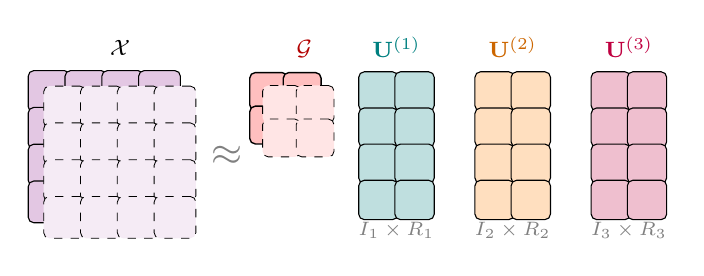
\begin{tikzpicture}[scale=0.82, every node/.style={font=\small}]
  % Tensor X
  \begin{scope}[xshift=0cm]
    \def\dx{0.24}\def\dy{-0.24}
    \foreach \s in {0,...,1}
      \foreach \i in {0,...,3}
        \foreach \j in {0,...,3}{
          \pgfmathsetmacro\bx{\j*0.57+\s*\dx}
          \pgfmathsetmacro\by{-\i*0.57+\s*\dy}
          \pgfmathtruncatemacro\ff{1-\s}
          \ifnum\ff=1
            \node[draw,fill=violet!22,minimum size=0.53cm,rounded corners=2pt,line width=0.4pt] at (\bx,\by) {};
          \else
            \node[draw,fill=violet!8,minimum size=0.53cm,rounded corners=2pt,line width=0.3pt,dashed] at (\bx,\by) {};
          \fi
        }
    \node[above,font=\footnotesize\bfseries] at (1.1,0.4) {$\mathcal{X}$};
  \end{scope}

  \node[font=\Large,gray] at (2.75,-1.0) {$\approx$};

  % Core G (nho hon)
  \begin{scope}[xshift=3.4cm]
    \def\dx{0.2}\def\dy{-0.2}
    \foreach \s in {0,...,1}
      \foreach \i in {0,...,1}
        \foreach \j in {0,...,1}{
          \pgfmathsetmacro\bx{\j*0.52+\s*\dx}
          \pgfmathsetmacro\by{-\i*0.52+\s*\dy}
          \pgfmathtruncatemacro\ff{1-\s}
          \ifnum\ff=1
            \node[draw,fill=red!25,minimum size=0.48cm,rounded corners=2pt,line width=0.5pt] at (\bx,\by) {};
          \else
            \node[draw,fill=red!10,minimum size=0.48cm,rounded corners=2pt,line width=0.3pt,dashed] at (\bx,\by) {};
          \fi
        }
    \node[above,font=\footnotesize\bfseries,red!70!black] at (0.55,0.38) {$\mathcal{G}$};
  \end{scope}

  % times_1 U1
  \begin{scope}[xshift=5.1cm]
    \node[font=\footnotesize] at (0,-0.5) {$\times_1$};
    \foreach \i in {0,...,3}
      \foreach \j in {0,...,1}
        \node[draw,fill=teal!25,minimum size=0.5cm,rounded corners=2pt] at (\j*0.56,-\i*0.56) {};
    \node[above,font=\footnotesize\bfseries,teal] at (0.28,0.38) {$\mathbf{U}^{(1)}$};
    \node[below,font=\scriptsize,gray] at (0.28,-3*0.56-0.2) {$I_1\times R_1$};
  \end{scope}

  % times_2 U2
  \begin{scope}[xshift=6.9cm]
    \node[font=\footnotesize] at (0,-0.5) {$\times_2$};
    \foreach \i in {0,...,3}
      \foreach \j in {0,...,1}
        \node[draw,fill=orange!25,minimum size=0.5cm,rounded corners=2pt] at (\j*0.56,-\i*0.56) {};
    \node[above,font=\footnotesize\bfseries,orange!80!black] at (0.28,0.38) {$\mathbf{U}^{(2)}$};
    \node[below,font=\scriptsize,gray] at (0.28,-3*0.56-0.2) {$I_2\times R_2$};
  \end{scope}

  % times_3 U3
  \begin{scope}[xshift=8.7cm]
    \node[font=\footnotesize] at (0,-0.5) {$\times_3$};
    \foreach \i in {0,...,3}
      \foreach \j in {0,...,1}
        \node[draw,fill=purple!25,minimum size=0.5cm,rounded corners=2pt] at (\j*0.56,-\i*0.56) {};
    \node[above,font=\footnotesize\bfseries,purple] at (0.28,0.38) {$\mathbf{U}^{(3)}$};
    \node[below,font=\scriptsize,gray] at (0.28,-3*0.56-0.2) {$I_3\times R_3$};
  \end{scope}
\end{tikzpicture}
\caption{Phân rã Tucker: tensor $\mathcal{X}$ được xấp xỉ bởi core tensor $\mathcal{G}$ nhỏ hơn và $N$ factor matrices $\mathbf{U}^{(n)}$. Core tensor mô tả tương tác giữa các mode; factor matrices chiếu mỗi mode xuống không gian con chiều thấp hơn.}
\label{fig:tucker-decomp}
\end{figure}

\begin{proposition}[Mối quan hệ Tucker -- CP]
Phân rã CP là trường hợp đặc biệt của Tucker với $R_1 = R_2 = \cdots = R_N = R$ và core tensor $\mathcal{G}$ là \textit{superdiagonal} (tức là $\mathcal{G}_{r_1,\ldots,r_N} = \lambda_r$ nếu $r_1 = \cdots = r_N = r$, và bằng 0 trong các trường hợp khác).
\end{proposition}

\begin{proof}
Với $\mathcal{G}$ superdiagonal và $\lambda_r = 1$:
\begin{equation}
    \mathcal{X}_{i_1,\ldots,i_N} = \sum_{r_1}\cdots\sum_{r_N} \mathcal{G}_{r_1,\ldots,r_N} \prod_{n=1}^N U^{(n)}_{i_n,r_n}
    = \sum_{r=1}^R \prod_{n=1}^N U^{(n)}_{i_n, r} = \sum_{r=1}^R \mathbf{u}^{(1)}_r \circ \cdots \circ \mathbf{u}^{(N)}_r,
\end{equation}
chính là phân rã CP với factor matrices $\mathbf{U}^{(n)}$.
\end{proof}

\subsubsection{HOSVD -- Thuật toán tính phân rã Tucker}

Thuật toán \textit{Higher-Order SVD} (HOSVD) \cite{delathauwer2000multilinear} là phương pháp tính phân rã Tucker đầu tiên và trực tiếp nhất:

\begin{enumerate}
    \item Với mỗi $n = 1, \ldots, N$: tính SVD của mode-$n$ matricization:
    \begin{equation}
        \mathbf{X}_{(n)} = \mathbf{U}^{(n)} \mathbf{\Sigma}^{(n)} (\mathbf{V}^{(n)})^\top.
    \end{equation}
    Lấy $R_n$ cột đầu của $\mathbf{U}^{(n)}$ làm factor matrix.
    \item Tính core tensor:
    \begin{equation}
        \mathcal{G} = \mathcal{X} \times_1 (\mathbf{U}^{(1)})^\top \times_2 (\mathbf{U}^{(2)})^\top \cdots \times_N (\mathbf{U}^{(N)})^\top.
    \end{equation}
\end{enumerate}

HOSVD cho xấp xỉ suboptimal nhưng đóng vai trò là điểm khởi tạo tốt cho các thuật toán tối ưu hóa như HOOI (Higher-Order Orthogonal Iteration).

%%============================================================
\subsection{Hạng tensor và độ phức tạp biểu diễn}
%%============================================================

\begin{definition}[Hạng CP và Tucker ranks]
\label{def:rank-cp-tucker}
Cho tensor $\mathcal{X} \in \mathbb{R}^{I_1 \times \cdots \times I_N}$.
\begin{itemize}
  \item \textit{Hạng CP} của $\mathcal{X}$: $\mathrm{rank}_{\mathrm{CP}}(\mathcal{X}) = \min\{R : \mathcal{X} = \sum_{r=1}^R \mathbf{a}^{(1)}_r \circ \cdots \circ \mathbf{a}^{(N)}_r\}$.
  \item \textit{Multilinear rank} (Tucker ranks): bộ $(R_1,\ldots,R_N)$ với $R_n = \mathrm{rank}(\mathbf{X}_{(n)})$.
\end{itemize}
\end{definition}

\begin{theorem}[NP-hardness của hạng tensor {\cite{hillar2013most}}]
Xác định hạng CP của một tensor bậc $N \geq 3$ là bài toán NP-hard.
\end{theorem}

Định lý này phân biệt căn bản tensor với ma trận: hạng ma trận tính được trong thời gian đa thức qua SVD, trong khi hạng tensor về nguyên tắc không thể tính hiệu quả. Đây là một trong những lý do tại sao nghiên cứu về phân rã tensor vẫn là lĩnh vực tích cực.

%%============================================================
\subsection{Phân rã tensor và tính đạo hàm bậc cao}
%%============================================================

Một động lực toán học tự nhiên cho tensor là \textit{tính tất yếu} của chúng trong giải tích đa biến. Cho $f: \mathbb{R}^n \to \mathbb{R}^m$ với $f(\mathbf{x}) = \mathbf{A}\mathbf{x}$ ($\mathbf{A} \in \mathbb{R}^{m\times n}$), đạo hàm theo ma trận $\mathbf{A}$ là:
\begin{equation}
    \frac{\partial f}{\partial \mathbf{A}} =
    \begin{pmatrix} \partial f_1 / \partial \mathbf{A} \\ \vdots \\ \partial f_m / \partial \mathbf{A} \end{pmatrix}
    \in \mathbb{R}^{m \times m \times n},
\end{equation}
là tensor bậc 3. Tổng quát hơn, đạo hàm bậc $k$ của một hàm đa biến tự nhiên tạo ra tensor bậc $k$. Điều này cho thấy tensor không phải là khái niệm ngoại lai mà là cấu trúc tất yếu trong giải tích và tối ưu hóa \cite{chrysos2025tutorial}.